% to compile this document use the following four commands: 
% pdflatex worms.tex
% bibtex worms.aux
% pdflatex worms.tex
% pdflatex worms.tex
\documentclass[12pt]{scrartcl}

% used packages
\usepackage{graphicx}
\usepackage{url}
\usepackage{listings}

% settings for listings
\lstset{language=Java}
\lstset{frame=single}
\lstset{framesep=10pt}
\lstset{basicstyle=\ttfamily}

% title, authors and date
\title{Oblig 2 \\ Creating a Domain Specific Language using the Eclipse Modelling Framework}
\author{Tobias Birmili, Florian Hagenauer, Kacper Surdy}

\date{07.05.2012}

\begin{document}

\maketitle

\tableofcontents

\section{Introduction}

This report is about the second assignment for the course "Modelbased System Development". It discusses how the three
parts of the assignment have been solved and implemented. The basic task was to design a model for customer journeys using
the Eclipse Modelling Framework\footnote{EMF - \url{http://www.eclipse.org/modeling/emf/}}, make it possible to extract 
statistics out of the customer journeys and finally the option to choose between three different tasks. For the third part 
it was possible to choose between a user-friendly editor, a graphical exporter or adding support for multiple journeys. In
this report, the third option, a graphical exporter, was chosen and combined with the statistic component.

The first Section \ref{section:model} describes how the model was built and discusses the different components. The next
section \ref{section:statistic} depicts which statistics were generated. Section \ref{section:export}
compares the initial graph idea to the final graphs produced by the exporter. Section \ref{section:merge} explains how
the statistic and the exporter components were merged to generate a useful HTML report. Finally, section \ref{section:impl} shows
some details about the implementation and how we used the EMF tools.

\section{Creating a DSL metamodel with EMF} 
\label{section:model}

The first part of the work was to create a metamodel using the Eclipse Modelling Framework for a customer
journey. A customer journey describes a collection of interactions a customer has with a product. These interactions are
so called touchpoints. Such a journey usually consists of a reference which describes how the interactions should ideally
look like. After finalizing this journey some customer are asked to take the journey and rate the different touchpoints and 
maybe add new ones for special interactions which have not been covered in the reference journey. Every touchpoint should 
be rated and, if possible, commented. For this metamodel, we had some example journeys consisting of a reference journey 
and four different customer journeys which differ in some ways from the reference. 

\subsection{Domain Specific Language Metamodel}
The model itself consists of three main components: The first one is the \lstinline!JourneySet!. This component
includes the reference journey and a set of examples. A reference journey has to be set to allow comparison
between the example journeys and the reference. This component also has a method which allows the comparison
of the journeys to the reference journey. The model also contains the method \lstinline!getComparedToExpectedJourney(Journey)!
which compares a given journey to the reference. Other methods generate the graphical export and the markdown source of the
statistics. More information on the two latter things can be found in Sections \ref{section:statistic} and \ref{section:export}.

The second component is the \lstinline!Journey! which depicts the Customer journey itself. This journey consists of 
an ID, a more descriptive name, a date, the status and an optional comment. If the ID of a journey is 
\lstinline!reference! then the journey is considered to be the reference journey. The model also contains some 
methods which allow to compare the journeys and generate statistics for a special journey or generate the graphical
representation. A more detailed description of this can also be found in the Sections \ref{section:statistic} and
\ref{section:export}.

The last main component is called \lstinline!Touchpoint!. It describes the users interaction and experience during
a journey. Beside an ID, a name, a date and a comment it also has a type which describes if it is a generic or
and ad-hoc touchpoint, and an evaluation where the customer votes how good the experience at the touchpoint was, a 
initiator for the touchpoint and finally a channel through which this touchpoint was experienced. The variables
channel, component, type, initiator and evaluation were done as enums. In that way they can be extended quite
easily by adding a new type to the enum and generate the code. The methods have been written as generic as possible
to allow easy extension of these enums.

Another part, which is important for \ref{section:statistic}, is the component \lstinline!JourneyDiff! which stores
the differences between the reference journey and the different example journeys.

\section{Making a Transformation to extract Statistics} 
\label{section:statistic}

The second task was to extend the model to generate statistics and print them in a convenient form. To represent
this generation in the model some methods were added to the \lstinline!JourneySet! and to the \lstinline!Journey!
components. The \lstinline!JourneySet! has the operation \lstinline!getComparedToExpected! to compare the example 
journeys from the set to the reference journey. The single journeys got methods which allow to extract single
statistics for the journey. These statistics are:
\begin{description}
	\item[Rating Statistic] These statistics scan the different rating types and allow to see how often each rating
	was given and the percentage of the total ratings.
	\item[Channel Statistics] These statistics cover the number of channels and their percentage.
	\item[Initiator Statistics] How often an initiator invoked touchpoints can be found in this statistic.
	\item[Compare To Reference] This statistic shows how much the example journey differ from the given reference
	journey.
\end{description}

One part of the assignment was to print the statistics in a convenient and useful way.
We choose the generate a HTML report which contains all data in a standalone file for easy sharing. The report
contains all the journeys with their touchpoints, the generated graphs and statistics. The list of touchpoints
is linked with the graphical representation by clientside scripting. This report is generated using markdown
Freemaker, a Java Templating Library. The statistics are converted from their plain text Markdown\footnote{http://daringfireball.net/projects/markdown/} representation to HTML and inserted. This allows to also
produce ACSII only or CLI output on the console which is still easy for a human to read. At the time
of writing this report the Analyzer component does not  produce the markdown source directly but the merged product as 
described in  section \ref{section:merge}. The classic markdown-only report can be easily activated again by doing
simple modifications to the source code.

\section{Graphical Export} 
\label{section:export}

The last part of the assignment was to choose between different extensions for the metamodel. In this article
the graphical export feature was chosen. The task was to generate a graphical representation of the customer
journeys to make them more easy to understand and analyze them. The choice in this article fell to the Graphviz framework 
\footnote{\url{http://graphviz.org/}} a visualization framework that allows to print graphs in a convenient way.
The metamodel was extended with the operation \lstinline!getGraphviz! inside of \lstinline!JourneySet! and
\lstinline!Journey!. The basic idea can be seen in Figure \ref{figure:sample_figure}.

\begin{figure}[hbtp]
	\centering
	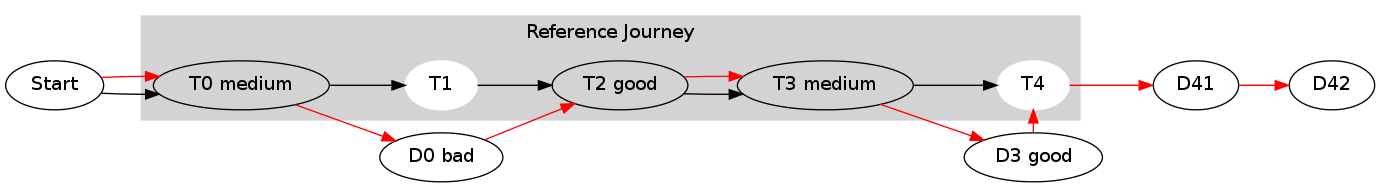
\includegraphics[scale=0.33]{img/sample_journey1.png}
	\caption{The basic idea for the visualization}
	\label{figure:sample_figure}
\end{figure}

The basic idea is to have the reference journey, here depicted in the grey box and the black arrows, and the 
example journey, which has red arrows in the example. It should be easy to spot the difference between the
reference and the example journey. Also the ratings are directly included into the graph.

Figure \ref{figure:sample_figure2} shows the same customer journey as Figure \ref{figure:sample_figure} but this
time the generated version. In the final version, instead of written ratings, colors are used (orange for
medium, red for bad and green for good). This makes it easier to see the general satisfaction. One rectangle always
shows the reference journey and another the new (mostly ad-hoc) touchpoints added by the example. Also, the orange
arrows make it easy to follow the example journey.

\begin{figure}[hbtp]
	\centering
	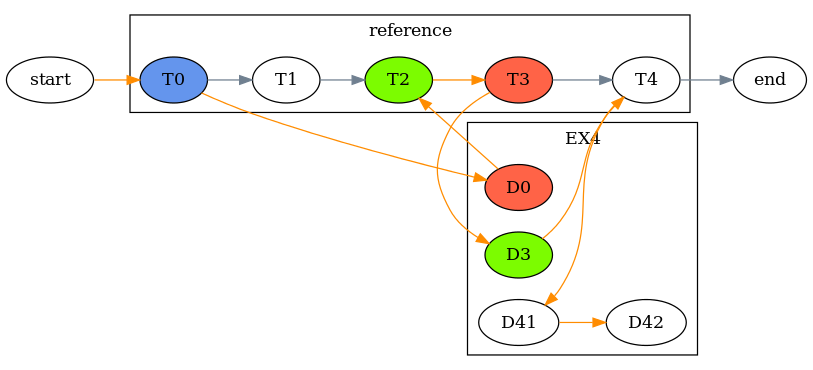
\includegraphics[scale=0.5]{img/sample_journey2.png}
	\caption{The realization generated by the Visualizer}
	\label{figure:sample_figure2}
\end{figure}

\section{Merging Graphical Export and Statistics}
\label{section:merge}

The last work done for this assignment was to merge the graphical export feature and the statistics view. This was
implemented into the Analyzer component and generates a new HTML file which can be viewed with a web browser (tested
with Chrome 18+, Firefox 12 and Safari). The HTML shows a tabbed view of all the example journeys and it is possible to view
every journey on its own. All the statistics from the analyzer can be found here. By hovering over a touchpoint
it is highlighted in the graphical export which allows an easy overview even of very complex journeys. The reverse
way is also possible.

Figure \ref{figure:merge_figure} shows an example of the merged component. Every page also shows the complete overview
and the touchpoints there are also highlighted. To generate the HTML the CLI from the Analyzer component has to be run
and a new HTML file named \lstinline!output.hmtl! is generated. This file can be viewed with any recent web browser.

\begin{figure}[hbtp]
	\centering
	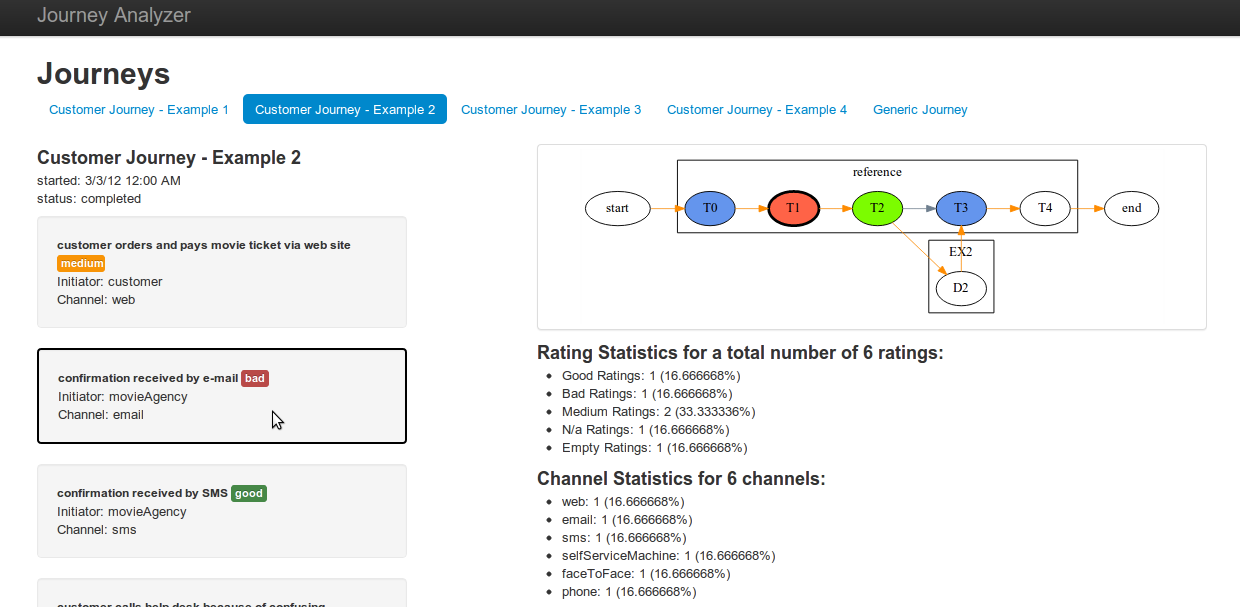
\includegraphics[scale=0.35]{img/merge_sample1.png}
	\caption{A screenshot of the merged components}
	\label{figure:merge_figure}
\end{figure}


\section{Implementation Details}
\label{section:impl}

In this section some details about the implementation and the general project can be found. Figure \ref{figure:projects} 
shows the different projects for the assignment. The project Customer Journey is the main project 
which contains the model and the generated code. The three projects .edit .editor and .tests are generated by the model. 
The .editor was used to define the example and the reference journeys. The project .analyzer contains the source code to 
load a customer journey set and return the analysis. Finally, the .visualizer project is responsible for visualizing the 
customer journeys as described in Section \ref{section:export}.

\begin{figure}[hbtp]
	\centering
	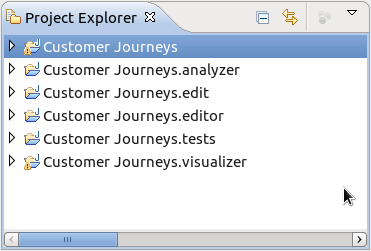
\includegraphics[scale=0.7]{img/projectexplorer.png}
	\caption{The different Eclipse projects of the assignment}
	\label{figure:projects}
\end{figure}

For version control and collaboration, a git repository hosted on Github was used\footnote{\url{https://github.com/floxyz/INF5120}}.

\end{document}
